%% Pretty formatted LaTeX/TikZ source
%% Fig09-SigmaDirectionalDiagrams.tex
%% Unused packages and definitions removed; TikZ/PGFPlots source formatted.

\documentclass[tikz,border=10pt]{standalone}
\usepackage{pgfplots}
\pgfplotsset{compat=1.17}
\input{../../definitions}

\begin{document}
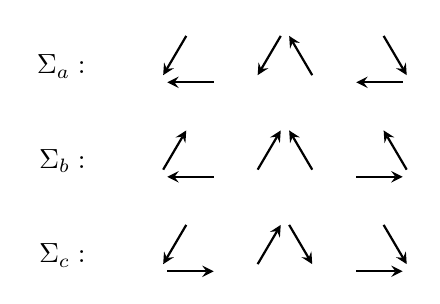
\begin{tikzpicture}[scale=0.2,thick,>=stealth,shorten >=3pt,shorten <=3pt]

    % ROW 1
    \begin{scope}[yshift=0cm,xshift=0cm]
        \coordinate (v1) at (-2,0);
        \coordinate (v2) at (0,3.4);
        \coordinate (v3) at (2,0);
        \draw[<-] (v1) to (v2);
        %\draw (v2) to (v3);
        \draw[->] (v3) to (v1);
    \end{scope}

    \begin{scope}[yshift=0cm,xshift=6cm]
        \coordinate (v1) at (-2,0);
        \coordinate (v2) at (0,3.4);
        \coordinate (v3) at (2,0);
        \draw[<-] (v1) to (v2);
        \draw[<-] (v2) to (v3);
        %\draw (v3) to (v1);
    \end{scope}

    \begin{scope}[yshift=0cm,xshift=12cm]
        \coordinate (v1) at (-2,0);
        \coordinate (v2) at (0,3.4);
        \coordinate (v3) at (2,0);
        %\draw (v1) to (v2);
        \draw[->] (v2) to (v3);
        \draw[->] (v3) to (v1);
    \end{scope}

    \begin{scope}[yshift=0cm,xshift=-6cm]
        \draw (0,1) node[anchor=east] {$\Sigma_a:$};
    \end{scope}

    % ROW 2
    \begin{scope}[yshift=-6cm,xshift=0cm]
        \coordinate (v1) at (-2,0);
        \coordinate (v2) at (0,3.4);
        \coordinate (v3) at (2,0);
        \draw[->] (v1) to (v2);
        %\draw (v2) to (v3);
        \draw[->] (v3) to (v1);
    \end{scope}

    \begin{scope}[yshift=-6cm,xshift=6cm]
        \coordinate (v1) at (-2,0);
        \coordinate (v2) at (0,3.4);
        \coordinate (v3) at (2,0);
        \draw[->] (v1) to (v2);
        \draw[<-] (v2) to (v3);
        %\draw (v3) to (v1);
    \end{scope}

    \begin{scope}[yshift=-6cm,xshift=12cm]
        \coordinate (v1) at (-2,0);
        \coordinate (v2) at (0,3.4);
        \coordinate (v3) at (2,0);
        %\draw (v1) to (v2);
        \draw[<-] (v2) to (v3);
        \draw[<-] (v3) to (v1);
    \end{scope}

    \begin{scope}[yshift=-6cm,xshift=-6cm]
        \draw (0,1) node[anchor=east] {$\Sigma_b:$};
    \end{scope}

    % ROW 3
    \begin{scope}[yshift=-12cm,xshift=0cm]
        \coordinate (v1) at (-2,0);
        \coordinate (v2) at (0,3.4);
        \coordinate (v3) at (2,0);
        \draw[<-] (v1) to (v2);
        %\draw (v2) to (v3);
        \draw[<-] (v3) to (v1);
    \end{scope}

    \begin{scope}[yshift=-12cm,xshift=6cm]
        \coordinate (v1) at (-2,0);
        \coordinate (v2) at (0,3.4);
        \coordinate (v3) at (2,0);
        \draw[->] (v1) to (v2);
        \draw[->] (v2) to (v3);
        %\draw (v3) to (v1);
    \end{scope}

    \begin{scope}[yshift=-12cm,xshift=12cm]
        \coordinate (v1) at (-2,0);
        \coordinate (v2) at (0,3.4);
        \coordinate (v3) at (2,0);
        %\draw (v1) to (v2);
        \draw[->] (v2) to (v3);
        \draw[<-] (v3) to (v1);
    \end{scope}

    \begin{scope}[yshift=-12cm,xshift=-6cm]
        \draw (0,1) node[anchor=east] {$\Sigma_c:$};
    \end{scope}

\end{tikzpicture}

\end{document}

